% Section content template for individual Educative lessons
% This file contains the actual content for a specific section
% Generated from Educative API section content

% Section: Architectural Design Patterns
% Section ID: 5602661385502720
% Section Slug: architectural-design-patterns
% Generated: 2025-12-11T06:16:31.653899

\subsection{What are architectural design patterns?}\label{KwZ4BNyHtRLZl9YDBZyfP}
\\
\textbf{Architectural design} patterns help us decide how to structure an entire application or its large parts. These patterns give us a blueprint for organizing code to stay clean, flexible, and easy to maintain as the project grows. There are two main types of architectural patterns:

\begin{itemize}
\item
\protect\phantomsection\label{x9HhvhA0xmmRy8krF-ox2}
\textbf{UI architectural patterns:} These describe how to organize code inside the presentation layer(It is the application part that shows the user interface and handles user interactions.) of an app. They help separate the user interface, business logic, and data, making testing and updating each part easier without breaking the others. Some commonly used UI architectural patterns include MVC, MVP, and MVVM.
\item
\protect\phantomsection\label{3-BQNTVPx_xwyPboVHgtp}
\textbf{System-level architectural patterns} describe how the major parts of an application work together. Some common examples include layered architecture, microservices, client--server, and event-driven architecture.
\end{itemize}
\\
This lesson will focus on three popular UI architectural patterns: MVC, MVP, and MVVM. These patterns are widely used in web, desktop, and mobile app development.

\begin{figure}[htbp]
 \centering
 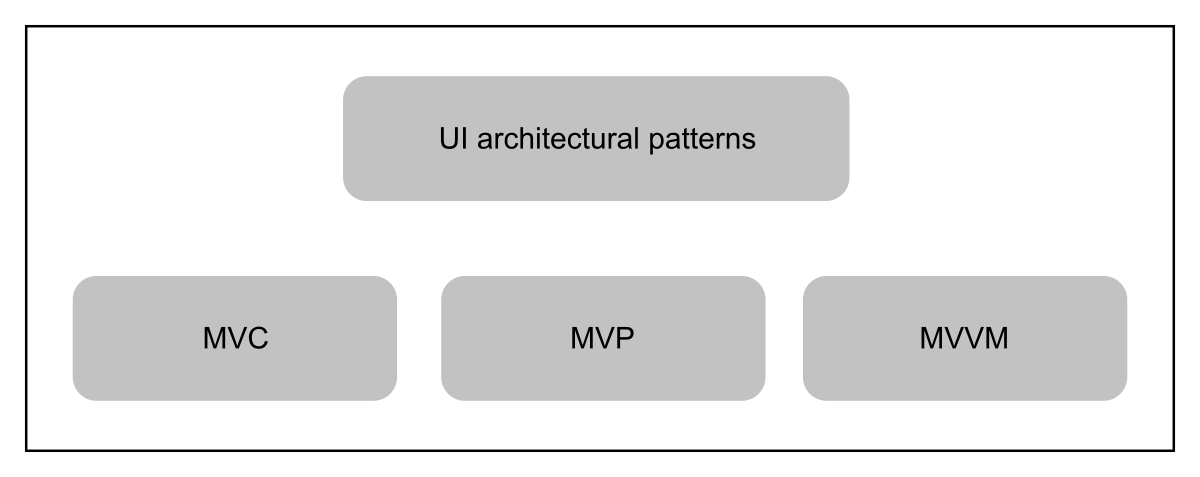
\includegraphics[width=0.5\textwidth]{Images/chapter_5/section_5602661385502720/6459627066490880.png}
 
\end{figure}

\subsection{Model-View-Controller (MVC)}\label{Bd_ZIKXr4_zNbek_N557r}
\\
\textbf{MVC (Model-View-Controller)} is a widely used architectural pattern in software design, especially for building user interfaces and web applications. It separates an application into three interconnected components:

\begin{itemize}
\item
\protect\phantomsection\label{d_ypz1DuwKPtOLZgdIP4p}
\textbf{Model:} It handles the data and business logic of the application. It is responsible for managing the rules of the application, storing and retrieving data from a database, and performing any calculations or operations needed. The Model does not care how the data is displayed; it only cares about the data and rules.
\item
\protect\phantomsection\label{ax1Vqsq3BY1rw2E6jjjLP}
\textbf{View:} It is the user interface that shows the data. It displays the data provided by the Model and presents it in a format that is easy for users to read and interact with. The View does not store any data by itself; it just shows what the Model gives it. If the data changes, the View updates to show the new information.
\item
\protect\phantomsection\label{DRa1yZTV6Rt1bkCeqHTT0}
\textbf{Controller:} It handles user input and interactions and bridges the View and the Model. When a user clicks a button or submits a form, the Controller takes this input, tells the Model what to do with it (like saving new data), and then decides which View should be shown next or how the View should be updated.
\end{itemize}
\\
In a web app, the HTML page is the View, the database and business rules are the Model, and the routes or handlers are the Controller. When a user clicks a button, the Controller updates the Model, and the View shows the latest data. This pattern is helpful when we want to keep UI and logic separate so that we can update one without affecting the other.

\subsection{Model-View-Presenter (MVP)}\label{FAB-oTFgLdV2dfq6ydHjP}
\\
The \textbf{Model-View-Presenter (MVP)} pattern is similar to MVC but replaces the Controller with a \textbf{Presenter}. The Presenter handles all the logic for the View.
\\
In MVP:

\begin{itemize}
\item
\protect\phantomsection\label{ljIE7InVXvNgUKHZski0h}
\textbf{Model:} It holds the data and contains the business logic. It manages the application's data, rules, and operations like in MVC. The Model does not know how the data is shown to the user.
\item
\protect\phantomsection\label{LNu0hOSTGn6Wr7A8DSdzM}
\textbf{View:} It is the user interface. It displays the data to the user and sends user actions (like button clicks or form submissions) to the Presenter. The View is usually kept as simple as possible and contains no business logic.
\item
\protect\phantomsection\label{TmB98Vdo1OFRuHN1y2Grs}
\textbf{Presenter:} It is the middle layer between the View and the Model. It talks to the Model to get the required data and then updates the View with that data. The Presenter also handles user input by deciding what to do when the user interacts with the View. Unlike the Controller in MVC, the Presenter usually has more control over the View and can tell it exactly what to display.
\end{itemize}
\\
In an Android app, the screen is the View, the data classes are the Model, and the Presenter handles what happens when the user clicks a button or enters text. This pattern is useful when writing unit tests for the logic without testing the actual UI.

\subsection{Model-View-ViewModel (MVVM)}\label{0JDw6qDtWyklzhV8D8ScJ}
\\
The \textbf{Model-View-ViewModel (MVVM)} pattern goes a step further. It adds a \textbf{ViewModel} that prepares and manages data for the View.
\\
In MVVM:

\begin{itemize}
\item
\protect\phantomsection\label{lK4FR59UWDg0QNhdfFBzS}
\textbf{Model:} It holds the application's raw data and business logic. It manages the data, makes network or database calls, and does not know how the data is shown on the screen.
\item
\protect\phantomsection\label{SkLlnAdo2G4D2QjKNGFW2}
\textbf{View:} The user interface displays the data on the screen so the user can see and interact with it. The View is kept as simple as possible and contains no business logic. Its job is only to show what the ViewModel provides and to forward user actions.
\item
\protect\phantomsection\label{z4JgAwjS_iWkclYQTuAVO}
\textbf{ViewModel:} It sits between the View and the Model. It gets data from the Model and prepares it in a format easy for the View to display. The ViewModel also contains the presentation logic and handles commands and actions from the View, like button clicks. Unlike the Presenter in MVP, the ViewModel does not directly control the View; instead, data binding is often used so that changes in the ViewModel automatically update the View.
\end{itemize}
\\
A key idea in MVVM is \textbf{data binding}. This allows changes in the ViewModel's data to be automatically reflected in the View, without needing extra update code. For example, in frameworks like WPF or Xamarin, you might have a \texttt{ViewModel} containing a \texttt{UserProfile} with properties such as \texttt{Name} and \texttt{ProfilePicture}. The View (often defined in XAML) directly binds its text boxes and image controls to these properties. If a user updates their name in the form, data binding also ensures the ViewModel is updated. Likewise, any changes made in the ViewModel, like loading a new profile picture, are instantly shown in the View, all without manually refreshing the UI.
\\
MVVM is especially useful for applications where the user interface wants to stay in sync with the underlying data automatically. It saves you from writing repetitive code to update the UI.

\subsection{Comparing MVC, MVP, and MVVM}\label{cvrDEw4JrqMK3Ta8ubJnE}
\\
Although these patterns all share the same goal of separating the user interface, logic, and data, MVC, MVP, and MVVM handle the flow between these parts in slightly different ways.

\begin{center}
{\def\LTcaptype{none} % do not increment counter
\begin{longtable}[]{@{}
>{\centering\arraybackslash} p{(\linewidth - 4\tabcolsep) * \real{0.3333}}
>{\centering\arraybackslash} p{(\linewidth - 4\tabcolsep) * \real{0.3333}}
>{\centering\arraybackslash} p{(\linewidth - 4\tabcolsep) * \real{0.3333}}@{}}
\toprule\noalign{}
\endhead
\bottomrule\noalign{}
\endlastfoot
\begin{minipage}[t]{\linewidth}\centering
\textbf{Pattern}
\end{minipage} & \begin{minipage}[t]{\linewidth}\centering
\textbf{How It Works}
\end{minipage} & \begin{minipage}[t]{\linewidth}\centering
\textbf{Example (Save Button)}
\end{minipage} \\
\begin{minipage}[t]{\linewidth}\centering
\textbf{MVC}
\end{minipage} & \begin{minipage}[t]{\linewidth}\centering
The controller handles user input and updates the Model. When the view needs to show updated information, it pulls data directly from the Model.
\end{minipage} & \begin{minipage}[t]{\linewidth}\centering
User clicks Save → Controller updates Model → View fetches saved data from Model and displays it.
\end{minipage} \\
\begin{minipage}[t]{\linewidth}\centering
\textbf{MVP}
\end{minipage} & \begin{minipage}[t]{\linewidth}\centering
View sends user actions to the Presenter. The Presenter updates the Model and directly tells the View what to display.
\end{minipage} & \begin{minipage}[t]{\linewidth}\centering
User clicks Save → View calls Presenter → Presenter updates Model → Presenter updates View with new data.
\end{minipage} \\
\begin{minipage}[t]{\linewidth}\centering
\textbf{MVVM}
\end{minipage} & \begin{minipage}[t]{\linewidth}\centering
View is bound to the ViewModel. The ViewModel updates the Model and automatically keeps the View in sync using data binding.
\end{minipage} & \begin{minipage}[t]{\linewidth}\centering
User clicks Save → ViewModel updates Model → Bound View updates itself automatically with new data.
\end{minipage} \\
\end{longtable}
}
\end{center}

\subsection{When to use architectural design patterns}\label{_PqgLzmxtVXSc0LoMA5YE}
\\
Architectural design patterns help organize large applications by setting clear rules for how major system parts work together. Here are some examples of when to use some common architectural patterns.

\begin{center}
{\def\LTcaptype{none} % do not increment counter
\begin{longtable}[]{@{}
>{\centering\arraybackslash} p{(\linewidth - 2\tabcolsep) * \real{0.5000}}
>{\centering\arraybackslash} p{(\linewidth - 2\tabcolsep) * \real{0.5000}}@{}}
\toprule\noalign{}
\endhead
\bottomrule\noalign{}
\endlastfoot
\begin{minipage}[t]{\linewidth}\centering
\textbf{Pattern}
\end{minipage} & \begin{minipage}[t]{\linewidth}\centering
\textbf{When to Use}
\end{minipage} \\
\begin{minipage}[t]{\linewidth}\centering
\textbf{MVC (Model--View--Controller)}
\end{minipage} & \begin{minipage}[t]{\linewidth}\centering
• Great for web apps where user input, data, and UI must be kept separate.
\\
• It makes testing and maintaining code easier when the UI and logic change often.
\end{minipage} \\
\begin{minipage}[t]{\linewidth}\centering
\textbf{MVP (Model--View--Presenter)}
\end{minipage} & \begin{minipage}[t]{\linewidth}\centering
• Good for desktop and mobile apps where the presentation logic needs to be easily testable.
\\
• Useful when you want the View to be completely passive.
\end{minipage} \\
\begin{minipage}[t]{\linewidth}\centering
\textbf{MVVM (Model--View--ViewModel)}
\end{minipage} & \begin{minipage}[t]{\linewidth}\centering
• Best for apps that support data binding, like WPF, Xamarin, or modern frontend frameworks.
\\
• Helps automatically keep the UI in sync with the data without extra glue code.
\end{minipage} \\
\end{longtable}
}
\end{center}



% End of section content